\section{First Model and Architecture} \label{subsec: first model and architecture}
The first class of networks augments the results in~\cite{Stöwer21MA}. P. Stöwer's models rely on predefined rules, like

\begin{itemize}
\phantomsection
\label{enum: rule set}
	\item \texttt{Adjective → Noun}
	\item \texttt{Verb → Adjective}
	\item \texttt{Personal Pronoun → Verb}
	\item \texttt{Question word → Personal Pronoun}
\end{itemize}
for building the dataset backed by a word database containing the corresponding information. Starting point is the \cognitiveroom{}, which consists of a list reflecting the whole data. The training data was crafted in accordance by randomly choosing respectively one of the four rules above and within the word class by chance an example. This information is used to initialize a \onehot{} and is done for input and output of the network.

The goal was to attain results on the behavior of the model if it is extended by more rules and words. One can imagine this type of model as a graph (\figref{\ref{fig: first model graph}}).

\begin{figure}
    \centering
    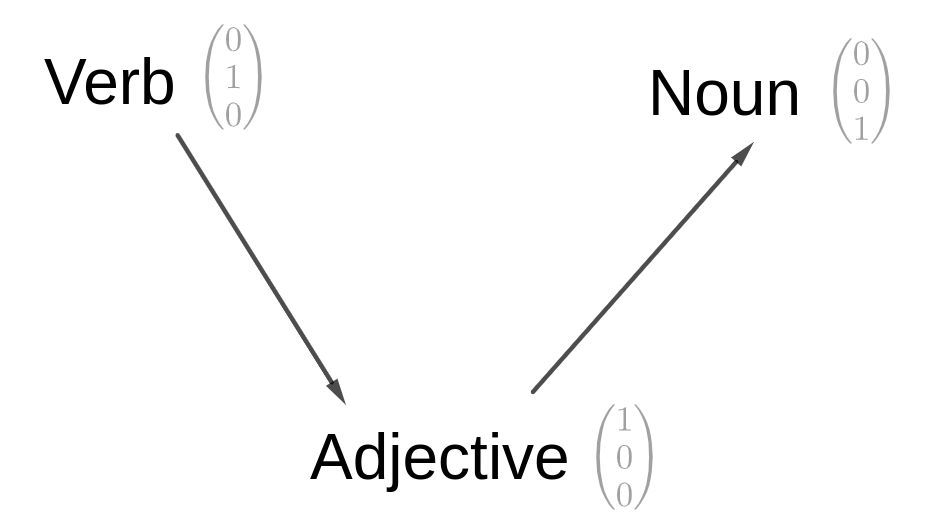
\includegraphics[scale=0.35]{Bilder/Graphen/first_model_graph2.png}
    \caption{The first two rules depicted as graph. In gray are corresponding \onehot{s} for the exemplary cognitive room \texttt{[blue, to run, desk]} denoted. The rules serve as edges and the word classes as vertices.}
    \label{fig: first model graph}
\end{figure}
